\subsection{Standard Model Single Top}
\label{sec:Bkg:SingleTop}

\indent Standard Model single top consists of 2 to 9 percent of the background in any one signal region $\RISR$ bin. Single top consist of 6 percent of the total background in the signal region.  A one lepton single top control region is defined in Table \ref{tab:ST1LCR}.  The single top control region is orthogonal to both the one lepton $W$+jets control region and $\ttbar$ control region.  \\

\begin{table}[h!]
  \begin{center}
    \begin{tabular}{c|c}
      \hline \hline
       { \bf Variables } & Single top 1 lepton control region           \\ \hline
      Number of leptons             & 1                                            \\ 
      Number of jets (incl. lepton) & $\geq 4$                                     \\ 
      $\pt$ of jets (incl. lepton)  & (80,80,40,40) GeV                            \\ 
      \mindphijettwomet             & $> 0.4$                                      \\ \
      $\met$                        & $>250$ GeV                                   \\ \hline
      \mtlepmet                     & $>30$,$<100$ GeV \\ 
      Number of $b$-jets            & $\ge2$                          \\ 
      \mantikttwelvezero            & v$>120$ GeV       \\
      \mtbmin                       & $>200\,$GeV   \\ 
      \mindrblep                    & $>2.0$             \\ 
      \drbjetbjet                   & $>1.5$               \\ \hline \hline
    \end{tabular}
  \end{center}
  \caption{Selection for the one lepton single top control region.  The one lepton preselection defined in Table \ref{tab:1Lcommon} is also applied.}
  \label{tab:ST1LCR}
\end{table}

\indent The lepton is treated as a jet for the jet multiplicity and the jet $\pt$ requirement as well as for the top reconstruction.  Similar to the one lepton $\ttbar$ control region, the lepton is meant to play the role of a hadronic tau jet in the zero-lepton signal region. \\

\indent $\mtlepmet$ is defined in equation \ref{eqn:mtlep} as the transverse mass of the lepton and the $\met$.  The $\mtlepmet$ selection ensures that the transverse mass is consistent with a $W$ decay.  \\

\indent The $\drbjetbjet$ variable is defined in equation \ref{eqn:drbb} as the $\Delta R$ between the two b-jets with the highest b-tagging values.  $\drbjetbjet > 1.5$ isolates single top events and rejects $\ttbar$.  This gives the single top control region a purity of $\sim50\%$. \\

\begin{equation}
\mindrblep = \sqrt{ \Delta\eta(b_1, b_2)^2 + \Delta\phi(b_1, b_2)^2}
\label{eqn:mindrblep}
\end{equation}

\indent The $\mantikttwelvezero > 120 \gev$ requirement selects for events with reconstructed boosted tops and ensures orthogonality with the $\Wjets$ control region.  $\mantikttwelvezero$ is defined as the mass of an $\antikt$ jet built with a distance parameter of $R=1.2$ instead of regular $R=0.4$.  The $\antikt$ algorithm clusters calorimeter energy into a jet according to the distance metric $R$ and is covered in detail in section \ref{sec:jet:reco}.  The large $R=1.2$ jet is designed to cluster all the energy of a boosted top quark into a single jet.  If the jet contains a boosted top, the invariant mass of jet should be close to $\sim m_t$.  \\

\indent $\mindrblep$ is defined in equation \ref{eqn:mindrblep} as the minimum $\Delta R$ between the two jets with the highest b-tag value and the selected lepton.  The $\mindrblep$ selection ensures orthogonality with the $\ttbar$ control region.  \\

\indent Kinematic distributions in the single control region are shown in figure ~\ref{fig:CRST}.  The MC background has been normalized to data by performing a simultaneous fit to all control regions.  The hashed bands on the total SM background correspond to the total experimental systematical uncertainty plus the MC statistical uncertainty.  The yield in the single top control region is given in table~\ref{table.bkgonly.CRST}.  \\

\indent  Data and MC are compatible to within statistical uncertainty.  No strong trends are observed in the data to MC ratios in any of the distribution. \\

%\begin{table}[!htb]
%  \centering
%  \begin{tabular}{c|c}
\hline\hline
\multicolumn{2}{c}{\bf CRST (44\% purity)} \\ \hline 
Z & 0.11 $\pm$ 0.05 \\
dibosons & 1.52 $\pm$ 0.54 \\
ttbar & 34.17 $\pm$ 2.10 \\
singleTop & 45.62 $\pm$ 1.41 \\
ttV & 2.42 $\pm$ 0.19 \\
W & 19.72 $\pm$ 1.69 \\
\hline
Total MC & 103.57 $\pm$ 3.10 \\
Data & 113.00 $\pm$ 10.63 \\
 \hline
SF & 1.21 $\pm$ 0.29 \\
\hline\hline
\end{tabular}

%  \caption{Yields in the CRST in $\intlumi$ $\ifb$ of data.  }
%  \label{tab:CRST}
%\end{table}

\begin{figure}[h!]
\begin{center}
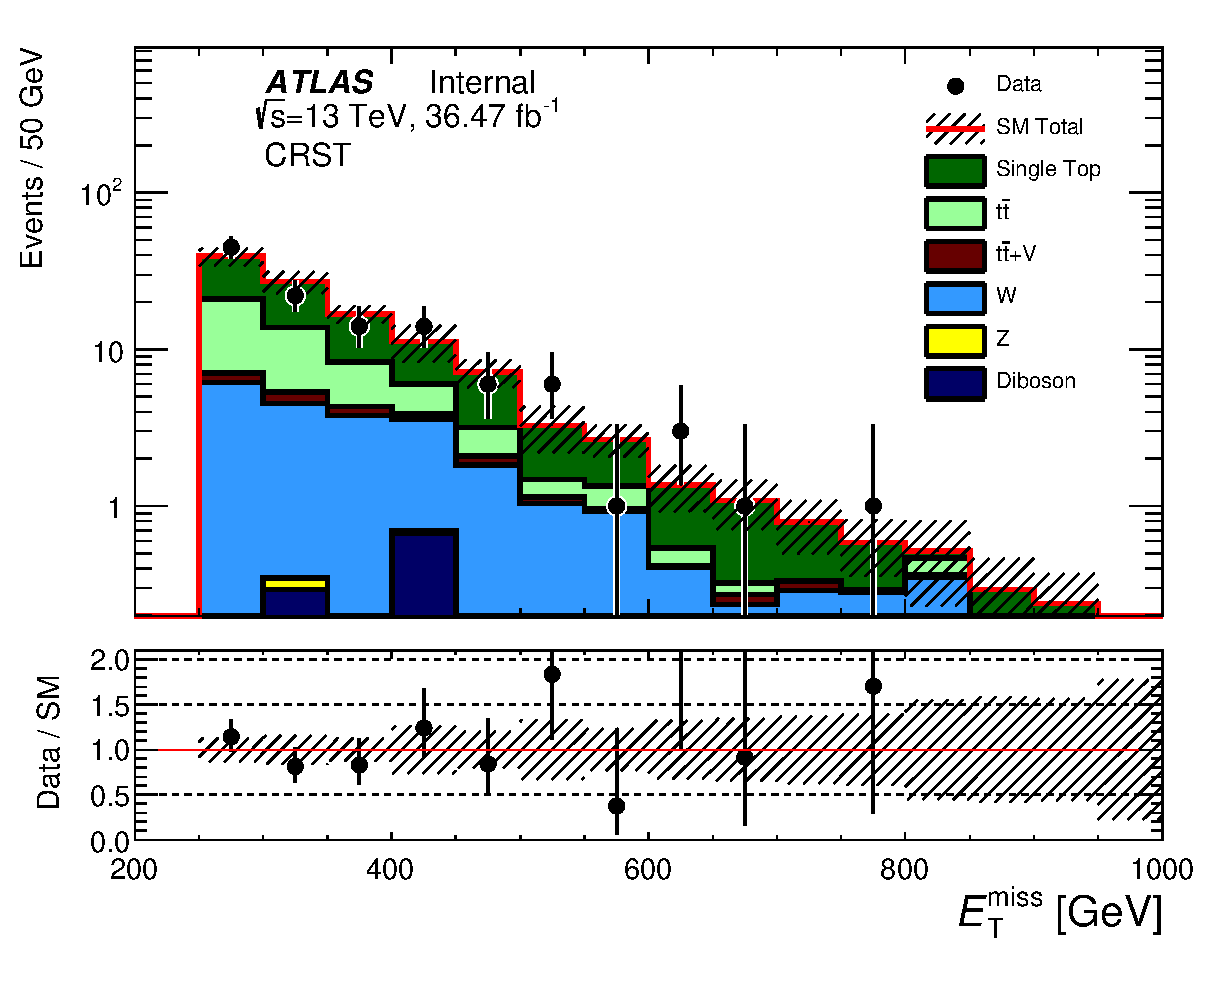
\includegraphics[width=0.45\textwidth]{figures/singleTop/postfit/Met_CRST_log.eps}
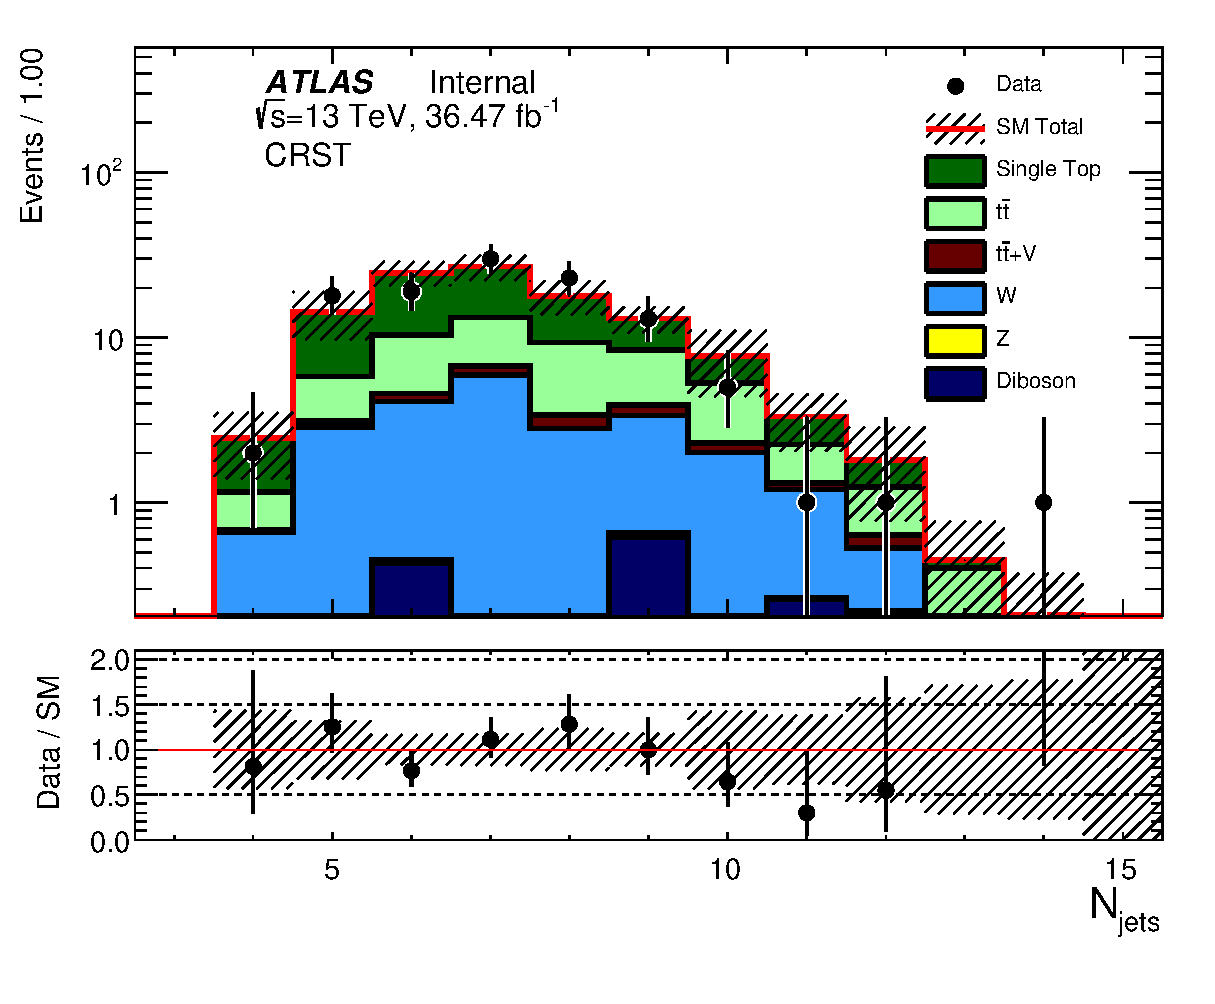
\includegraphics[width=0.45\textwidth]{figures/singleTop/postfit/NJets_CRST_log.eps}
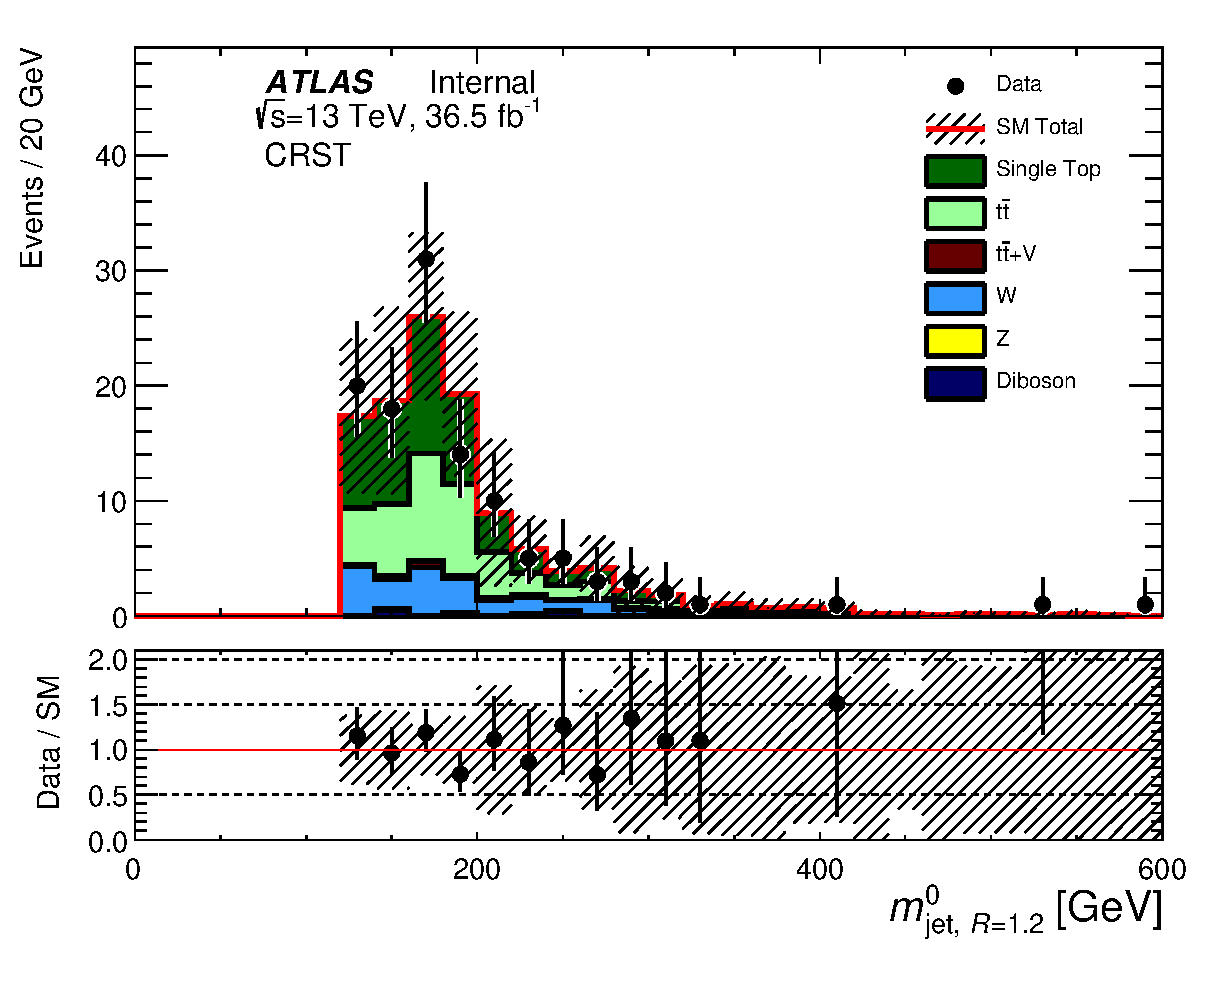
\includegraphics[width=0.45\textwidth]{figures/singleTop/postfit/AntiKt12M_0__CRST.eps}
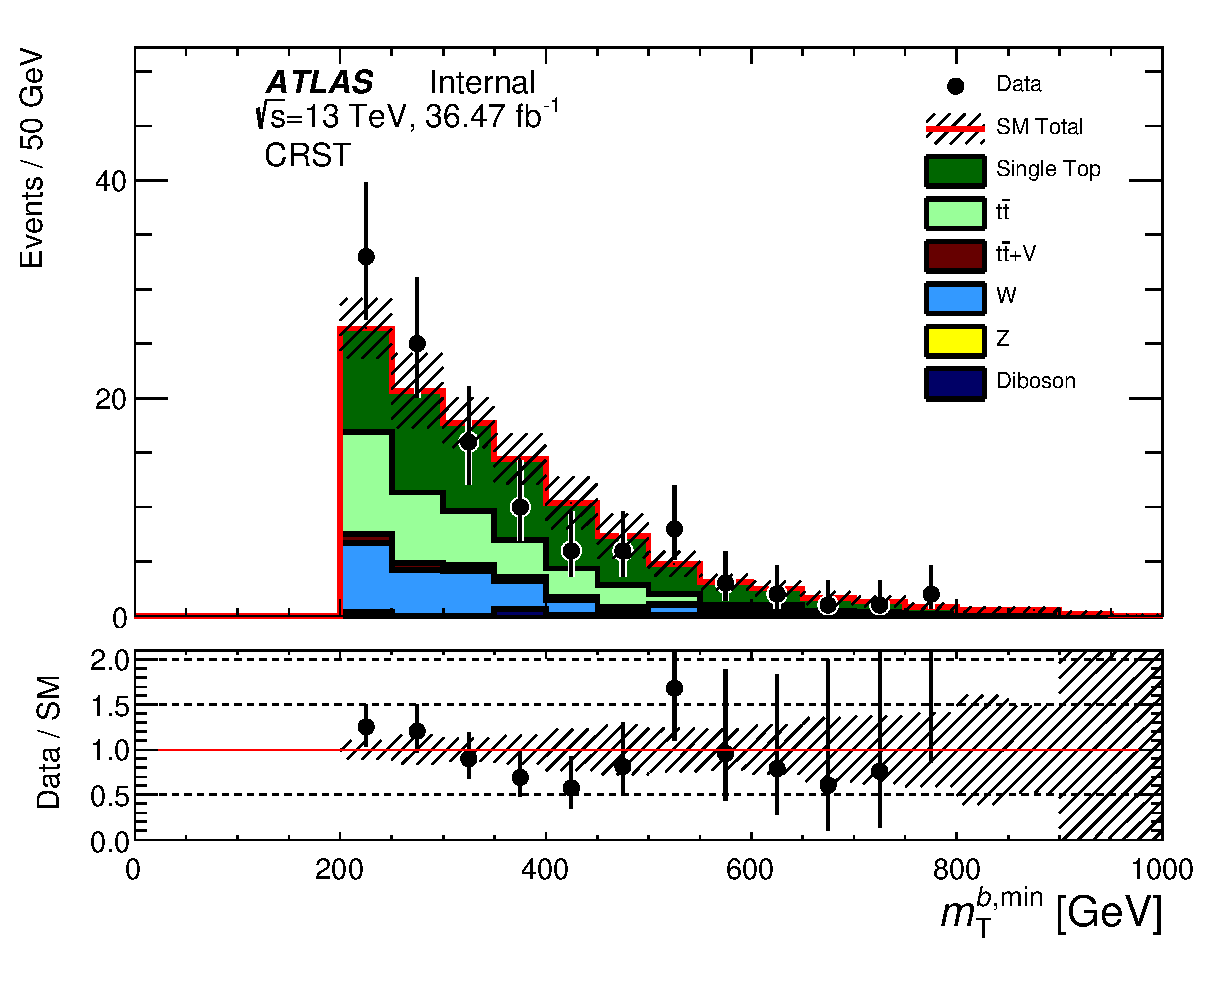
\includegraphics[width=0.45\textwidth]{figures/singleTop/postfit/MtBMin_CRST.eps}
%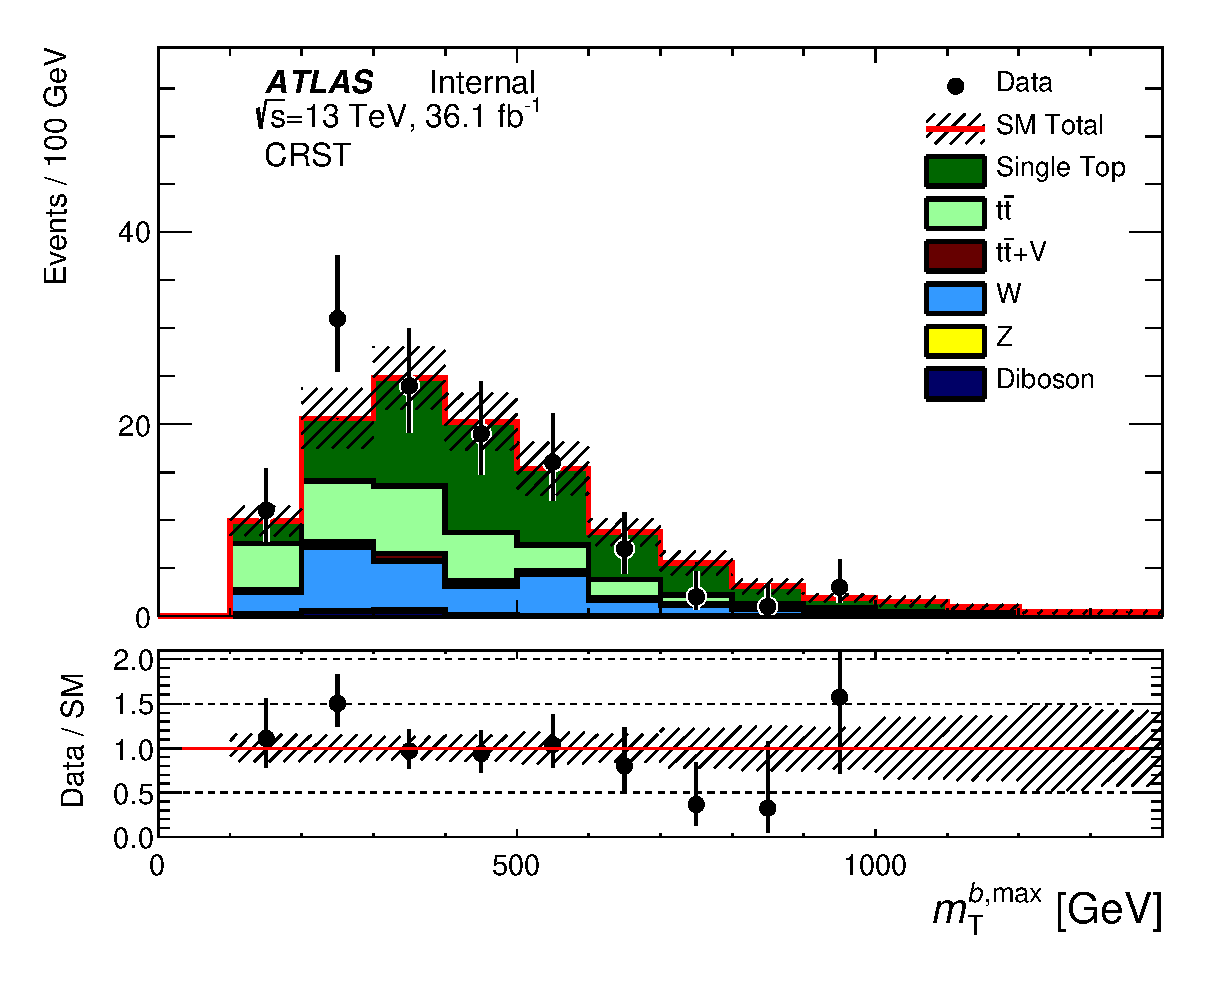
\includegraphics[width=0.45\textwidth]{figures/singleTop/postfit/MtBMax_CRST.eps}
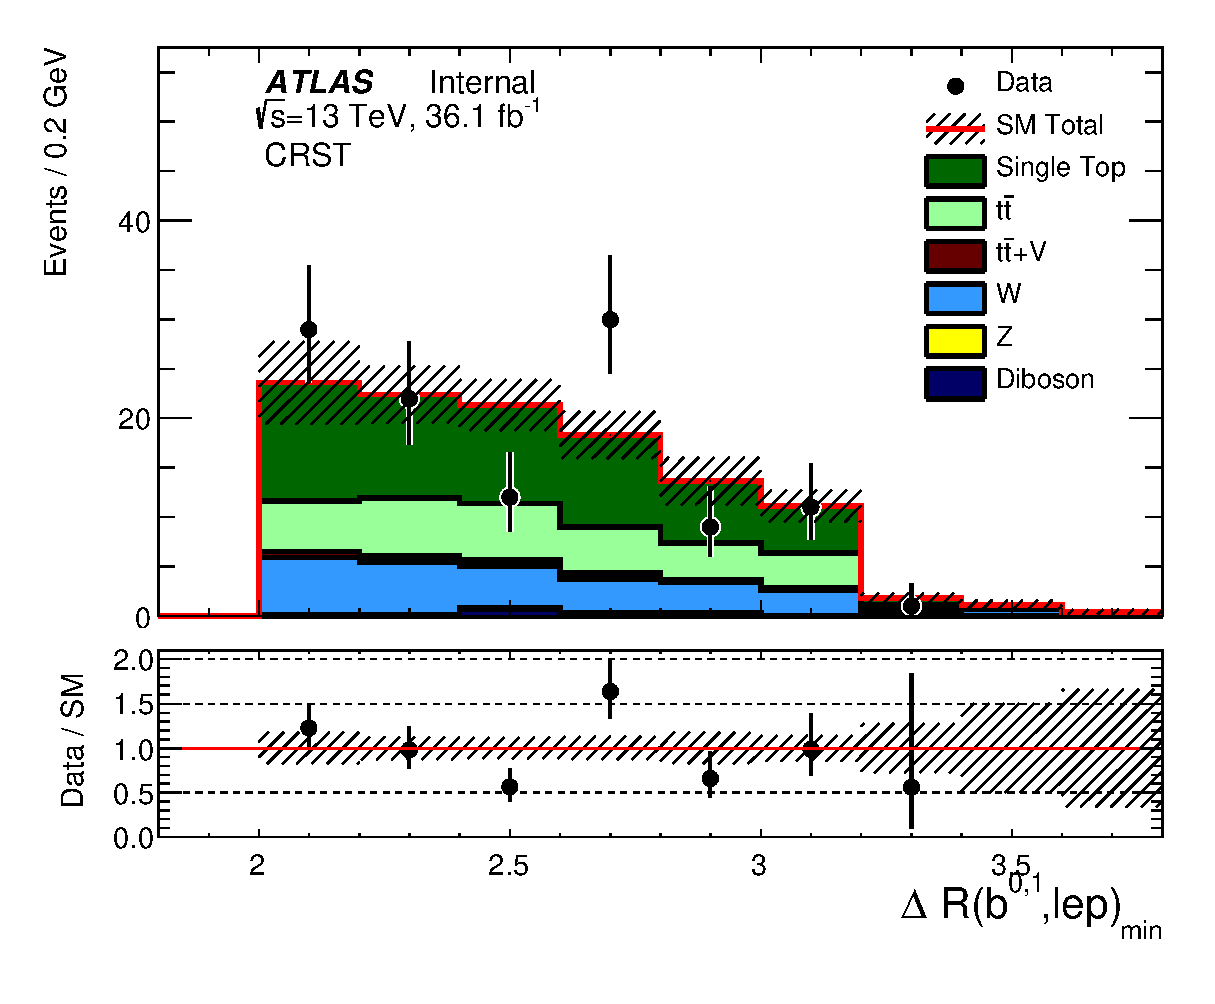
\includegraphics[width=0.45\textwidth]{figures/singleTop/postfit/MinDRBLep_CRST.eps}
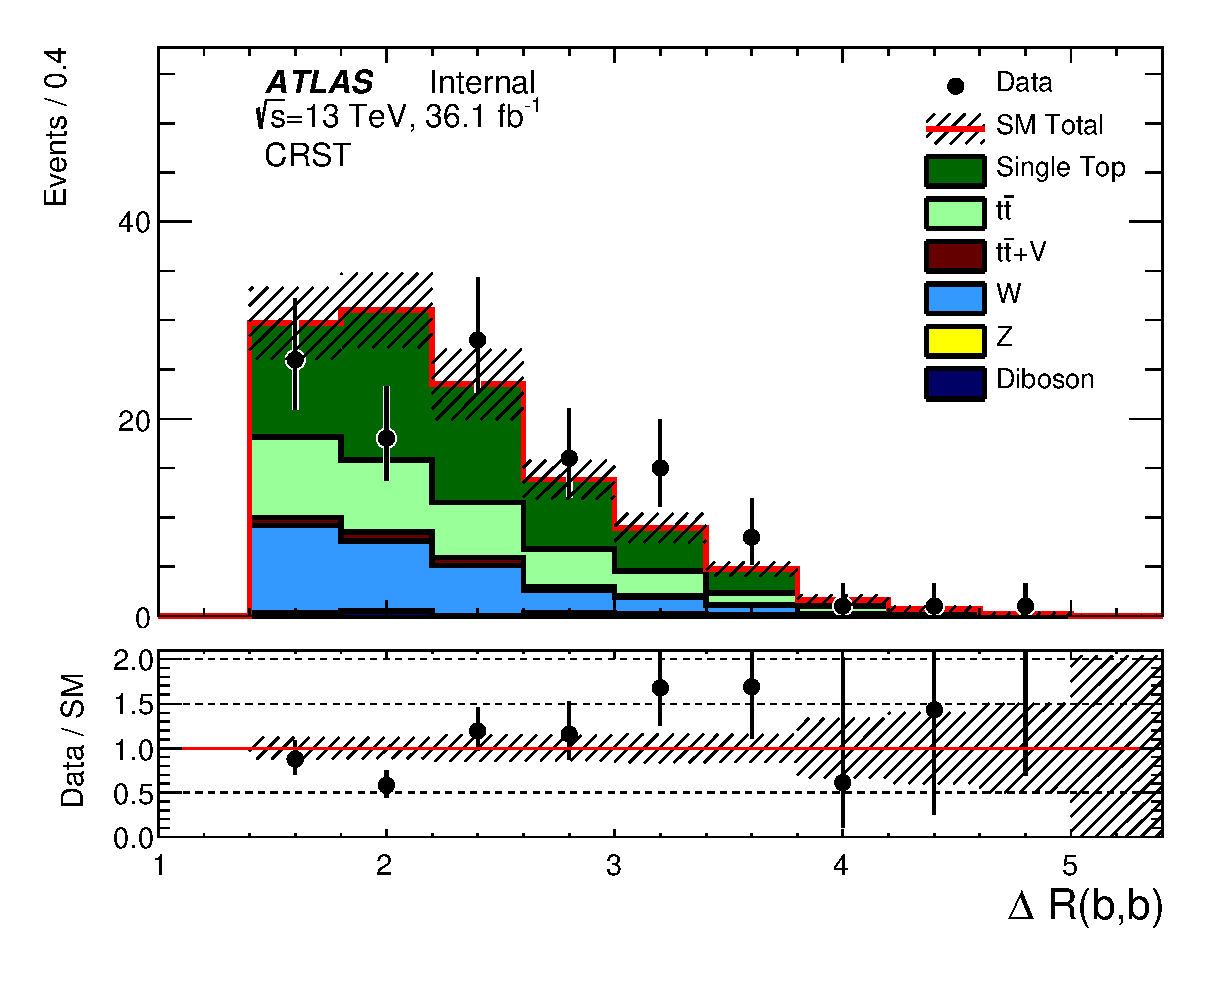
\includegraphics[width=0.45\textwidth]{figures/singleTop/postfit/DRBB_CRST.eps}
%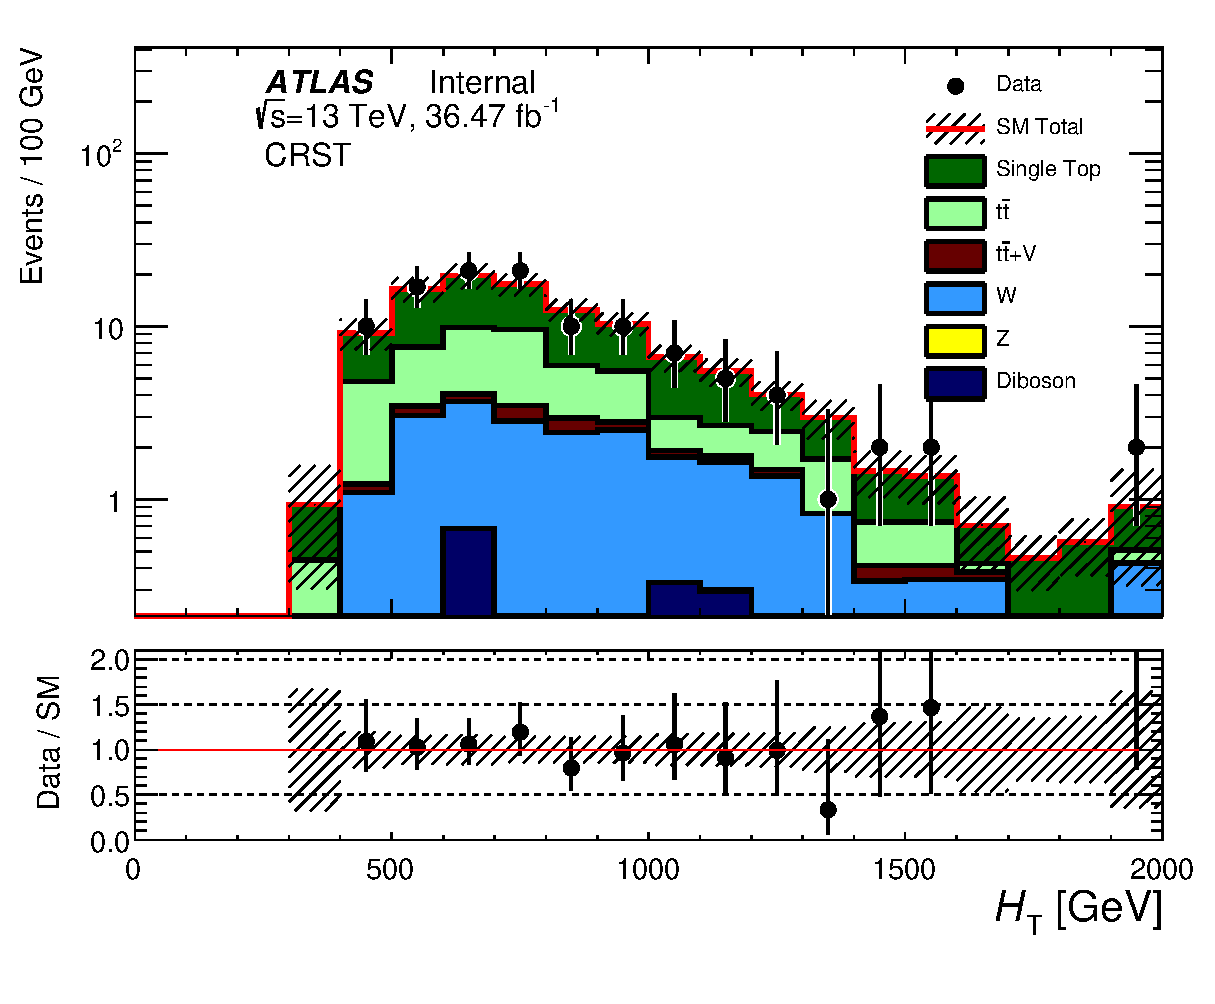
\includegraphics[width=0.45\textwidth]{figures/singleTop/postfit/Ht_CRST_log.eps}
%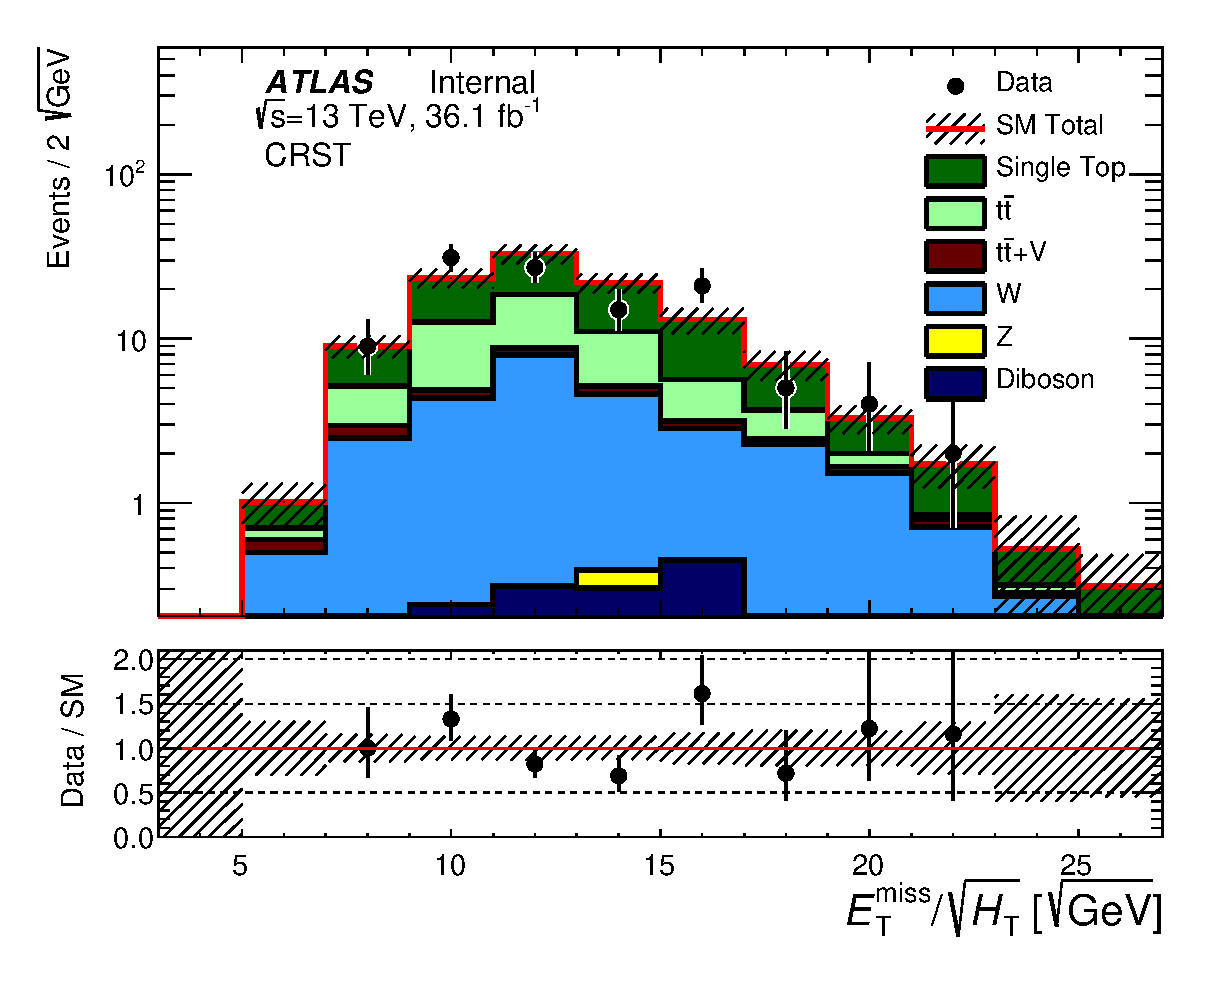
\includegraphics[width=0.45\textwidth]{figures/singleTop/postfit/HtSig_CRST_log.eps}
\end{center}
\caption[Single top control region distributions for $\intlumi$ $\ifb$ of data after a simultaneous fit to all control regions]{Single top control region distributions for \intlumi\ \ifb\ of data after a simultaneous fit to all control regions. The ratio between data and MC is shown in the bottom panel. The hashed area on the expected SM background represent the uncertainty due to experimental systematics and MC statistics.}
\label{fig:CRST}
\end{figure}



\begin{table}[h!]
\caption[$W$+jets control region MC Yield and background-only fit results for $\intlumi$ $\ifb$ of data]{$W$+jets control region MC Yield and background-only fit results for $\intlumi$ $\ifb$ of data. MC exp. events are expected background rates directly from MC predictions.  Fitted background event rates are the expected background rates after normalizing the MC to data by simultaneously fitting all control regions using a background only fit.  The fitted $W$+jets normalization scale factor is equal to (Fitted $\Wjets$ events)/(MC exp. $\Wjets$ events). The quoted uncertainties include statistical and systematic uncertainties. }
\label{table.bkgonly.CRW}
\begin{center}
\setlength{\tabcolsep}{0.0pc}
{\small
%%
\begin{tabular*}{\textwidth}{@{\extracolsep{\fill}}lr}
\noalign{\smallskip}\hline\noalign{\smallskip}
{\bf CRW yields}           & CRW                      \\[-0.05cm]
\noalign{\smallskip}\hline\noalign{\smallskip}
%%
Observed events          & $533$                       \\
\noalign{\smallskip}\hline\noalign{\smallskip}
%%
Fitted bkg events         & $533.23 \pm 23.09$                 \\
\noalign{\smallskip}\hline\noalign{\smallskip}
%%
        Fitted TTbar events         & $115.60 \pm 18.76$                     \\
%%
        Fitted Wjets events         & $349.54 \pm 38.87$                  \\
%%
        Fitted Zjets events         & $1.86 \pm 0.63$                   \\
%%
        Fitted TtbarV events         & $1.15 \pm 0.43$                     \\
%%
        Fitted SingleTop events         & $54.76 \pm 20.41$                     \\
%%
        Fitted Diboson events         & $10.31 \pm 2.34$                    \\
%%
        Fitted Multijets events         & $0.00 \pm 0.00$                 \\
%%     
 \noalign{\smallskip}\hline\noalign{\smallskip}
%%
MC exp. SM events              & $458.28 \pm 21.31$                     \\
\noalign{\smallskip}\hline\noalign{\smallskip}
%%
        MC exp. TTbar events         & $122.28 \pm 15.29$                   \\
%%
        MC exp. Wjets events         & $276.00 \pm 5.53$             \\
%%
        MC exp. Zjets events         & $1.79 \pm 0.52$                     \\
%%
        MC exp. TtbarV events         & $0.89 \pm 0.35$                      \\
%%
        MC exp. SingleTop events         & $47.00 \pm 5.70$                   \\
%%
        MC exp. Diboson events         & $10.31 \pm 2.35$                   \\
%%
        MC exp. Multijets events         & $0.00 \pm 0.00$                \\
%%     \\
\noalign{\smallskip}\hline\noalign{\smallskip}
Fitted $W$+jets normalization scale factor & $1.27 \pm 0.15$ \\
\noalign{\smallskip}\hline\noalign{\smallskip}
\end{tabular*}
%%%
}
\end{center}
\end{table}
%

